\documentclass{article}

% todo
% forum analysis
  % zotero export quote and reference it in the text
  % make a csv to read the entire forum
  % check a way of analysing into multiple categories

% observable
  % quantify the forum posts by categories, do a sitemap

% Notes
% Citation commands \cite \parencite \textcite 

% Useful packages
\usepackage[a4paper,top=2cm,bottom=2cm,left=3cm,right=3cm,marginparwidth=1.75cm]{geometry}
\usepackage{amsmath}
\usepackage{graphicx}
\graphicspath{{images/}}

\usepackage[colorlinks=true, allcolors=blue]{hyperref}
\usepackage[style=apa, backend=biber]{biblatex}
\addbibresource{main.bib}

\newcommand{\getyear}[1]{\citeyear{#1}}


\title{Charting the Beginnings of the Processing Community: Implications for Collaborative Open Source Art Development}
\author{Tibor Udvari}

\begin{document}

\maketitle

\begin{abstract}
What are the dynamics that lead to the creation of a community around a piece of software? How do these dynamics influence the development of the software itself? This thesis explores these questions through the lens of the Processing community, a community of artists and designers who use the Processing software to create interactive art. The paper traces the history of the Processing community from its beginnings in 2001 to the present day, using a combination of interviews, archival research, and analysis of the software development cycle itself. The paper finds that the Processing community was created through a combination of factors, including the software's design, the community's shared values, and the community's shared history. The paper also finds that the community's shared history has influenced the development of the software itself, with the community's values and history influencing the software's design. The paper concludes by discussing the implications of these findings for the development of collaborative open source art software.
\end{abstract}

%\tableofcontents

\section{Introduction}
\subsection{The Background and Importance of Open Source Projects}
% -- about open source communities in general
% -- importance of open source projects, maybe mention how flash died out, and the recent unity price change ?

\subsection{The Processing Project: A brief overview}
% todo - adapt to focus more on the research question

Processing was developed as a programming language and environment specifically tailored for the media arts communities. Its inception took place at the MIT Media Lab's Aesthetics and Computation Group (ACG) in 2001, led by Ben Fry and Casey Reas. Its foundational concepts build upon the earlier work from the Design By Numbers (DBN) programming platform, a project spearheaded by John Maeda \parencite{fryModernPrometheusHistory2018}.

Ben Fry shed light on the holistic nature of the Processing initiative, noting:
\begin{quote}
"The processing project is a community, a piece of software that you run, and a language. And that order is important."
\end{quote}
\parencite[19:22]{artsatmit2017CASTSymposium2017}

In its design philosophy, Processing introduced the concept of "software sketches". It was designed with an accessible entry point for beginners, while also providing advanced capabilities for experienced users \parencite{reasProcessingProgrammingMedia2006}.

Over the years, Processing has been adopted across various disciplines, showcasing its versatility. To further its impact and development, the Processing Foundation was established, with notable contributors like Daniel Shiffman. The foundation aims to support and expand the reach of the Processing software and its associated projects.

\subsection{Objective and Scope of the Research}
% Choice of processing, because the community has been around for a while and the project is still alive and taught in schools, also at a high school level

% modular toolkit, not a monolith
% community, application, syntax
% commercial software

\section{Literature review}
\subsection{Open Source Contributions: Historical Perspective and Modern Implications}
\subsection{Motivations behind Open Source Contributions}
\subsection{The intersection of Creative Coding and Open Source}
\subsection{Relevant Methodological Approaches in Computer Science and Anthropology}

\section{Methodology}

\subsection{Research Design}
\subsection{Quantitative Methods}
\subsubsection{ALPHA Forum Textual Analysis: Approach and Tools}
The research process began by manually reading the forum to identify themes and complemented with quantitative approaches. 
%todo forum composition

% todo
% check how much there is to read, estimate time
% relevance of the topics

\subsubsection{Forum Contributions Descriptive Statistics}

\subsection{Qualitative Methods}
\subsubsection{Interviews: Sample Selection, Interview Guide and Tools}


\section{Data Presentation and Analysis}

\subsection{Quantitative Findings}
\subsubsection{Trends in Git Commits}

Considering the \textit{Processing} project, its dependency on its primary contributor, Ben Fry, stands out as a potential vulnerability. Fry's instrumental role over the past two decades underscores the significance of his contributions. Were they to be unexpectedly interrupted, the project could face substantial challenges. This scenario exemplifies a high bus factor risk \parencite{BusFactor2023}, wherein the success and continuity of a project are profoundly dependent on a single, or very few, contributors. Such vulnerabilities appear to be common in open source projects, a sentiment humorously captured in popular culture and comics \parencite{munroeDependency2020}.

\begin{figure}[h!] 
    \centering
    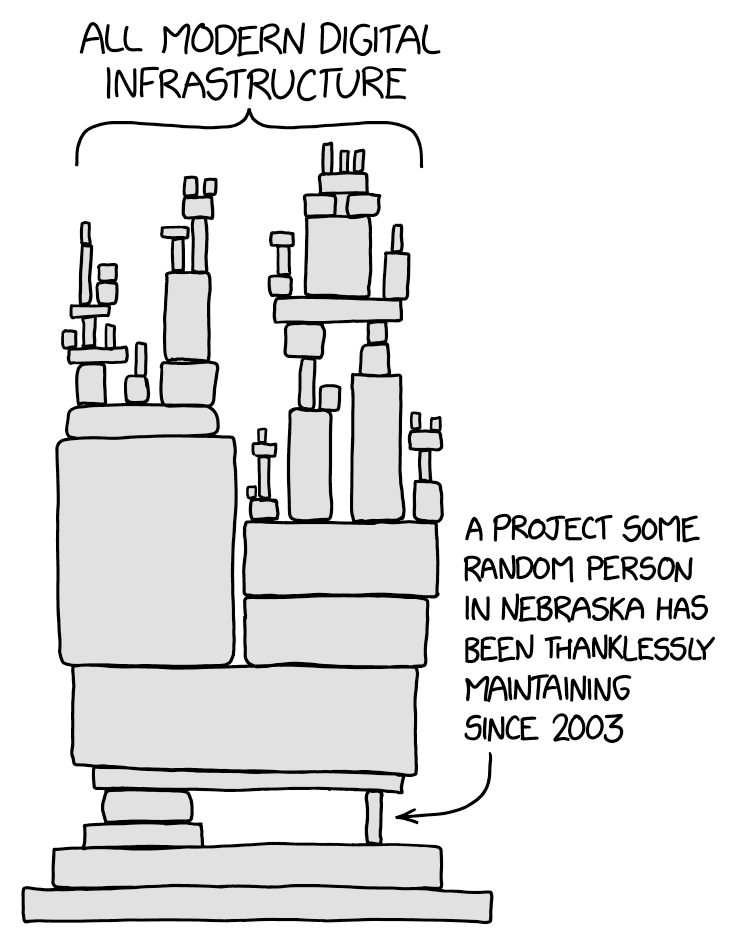
\includegraphics[width=0.75\textwidth]{dependency.png} 
    \caption{Dependency}
    \label{fig:dependency_comic}
    \small Source: \textit{XKCD}, \url{https://xkcd.com/2347/}, licensed under CC BY-NC 2.5.
\end{figure}

\subsubsection{Patterns in Forum Contributions}

\subsection{Qualitative Insights}
\subsubsection{Themes from the ALPHA Forum}
\subsubsection{Interview Highlights and Key Takeaways}

\section{Discussion}

\subsection{Integrating Quantitative and Qualitative Findings}
\subsection{Implications for the Open Source Community}
\subsection{The Unique Case of Processing and Creative Coding}
\subsection{Limitations of the Study}

\section{Conclusion and Recommendations}

\subsection{Recap of Key Findings}
\subsection{Practical Implications for Open Source Projects}
\subsection{Recommendations for Future Research}

\section{Acknowledgements}
I'm grateful to Randall Munroe of XKCD for his insightful and humorous comic strips. The comic "Dependency" from \getyear{munroeDependency2020} is in Figure~\ref{fig:dependency_comic} and cited as~\cite{munroeDependency2020}. It's under the Creative Commons Attribution-NonCommercial 2.5 License (CC BY-NC 2.5). License details: \url{https://creativecommons.org/licenses/by-nc/2.5/}.

\section{Bibliography}
\printbibliography

\section{Appendices}

\subsection{Interview Transcripts}

\section*{Interview Guide for Core Contributor}

\subsection*{Perceptions of Expertise and Community Role}

\begin{enumerate}
    \item Has your consistent involvement in resolving technical queries cultivated a sense of expertise or personal satisfaction for you?
    \item Can you comment on the emotional or psychological rewards, if any, you get from contributing?
    \item If you ceased your contributions tomorrow, what implications do you think that would have on the Processing project?
\end{enumerate}

\subsection*{Social Dynamics within the Community}

\begin{enumerate}[resume]
    \item How would you characterize the social fabric of the Processing community?
    \item Can you share an instance where the community's collective efforts resulted in something you alone couldn't have achieved?
    \item Have you ever experienced any conflicts within the community, and how were they resolved?
\end{enumerate}

\subsection*{Views on Technology and Development}

\begin{enumerate}[resume]
    \item What are your opinions on Flash and other proprietary technologies as they relate to Processing?
    \item Your contributions to Processing have been notably consistent. How do you interpret the fluctuating participation rates from others?
\end{enumerate}

\subsection*{Community and Open Source Development}

\begin{enumerate}[resume]
    \item What has been your observation regarding the community's growth, particularly concerning contributions to open source?
    \item Can you recall any "eureka moments" that significantly influenced the community's direction or ethos?
\end{enumerate}

\subsection*{Legacy and Continuation}

\begin{enumerate}[resume]
    \item How did p5 come into being as a continuation or evolution of Processing?
    \item What role did early literature play in legitimizing or boosting the project? Do you recall the impact of O'Reilly books or other publications?
\end{enumerate}

\section*{Interview Guide for Library Contributor}

\subsection*{Introduction and Motivation}

\begin{enumerate}
    \item What problem prompted you to contribute to Processing?
    \item How did you first hear about and decide to engage with the Processing community?
\end{enumerate}

\subsection*{Social Dynamics and Collaboration}

\begin{enumerate}[resume]
    \item Have you collaborated with other community members? What was that experience like?
    \item Were there any challenges in aligning your contributions with the broader community objectives?
\end{enumerate}
\subsection{Data Collection Tools and Scripts}

\begin{itemize}
    \item \href{https://forum.processing.org/alpha/}{Processing Alpha Forum}
    \item \href{https://observablehq.com/d/042b1cf42ea9bb5e}{Observable Notebook for Forum Analysis}
\end{itemize}


\subsection{List of Forum Threads Analyzed}


\end{document}